\documentclass[final]{beamer}
\usepackage[scale=1.2]{beamerposter}
\usepackage{graphicx}			% allows us to import images
%\newcommand{\degree}{\ensuremath{^\circ}}
\usepackage{lipsum}
\setlength{\paperwidth}{24in}
\setlength{\paperheight}{36in}
\setlength{\textwidth}{0.98\paperwidth}
\setlength{\textheight}{0.98\paperheight}
\setlength{\topmargin}{-0.25in}
\setlength{\tabcolsep}{22pt}

\newlength{\sepwid}
\newlength{\onecolwid}
\newlength{\twocolwid}
\newlength{\threecolwid}
\newlength{\fourcolwid}
\setlength{\onecolwid}{0.22\paperwidth}
\setlength{\twocolwid}{0.464\paperwidth}
\setlength{\threecolwid}{0.708\paperwidth}
\setlength{\fourcolwid}{0.952\paperwidth}



\usetheme{confposter}
\usepackage{exscale}
\newcommand\myheading[1]{%
  \par\smallskip
% {\Small\bfseries#1}\par\smallskip}
 {\Small\mdseries#1}\par\tinyskip}


%-----------------------------------------------------------
% Define colours (see beamerthemeconfposter.sty to change these colour definitions)
%-----------------------------------------------------------

\setbeamercolor{block title}{fg=nred,bg=white}
\setbeamercolor{block body}{fg=black,bg=white}
\setbeamercolor{block alerted title}{fg=yellow,bg=dblue!90}
\setbeamercolor{block alerted body}{fg=black,bg=dblue!10}

%-----------------------------------------------------------
% Name and authors of poster/paper/research
%-----------------------------------------------------------
%\logo{%
%    \includegraphics[width=4cm,height=4cm,keepaspectratio]{seedsower.png}~%
%}

\title{PyMOL Shortcuts For Faster Image Making}

%\title{Tools to ease the writing of scripts for figure making in PyMOL}
\author{\textbf{Blaine Mooers}}

\institute{\normalsize{Department of Biochemistry and Molecular Biology \& Laboratory of Biomolecular Structure and Function \\ University of Oklahoma Health Sciences Center, Oklahoma City, OK 73104\\blaine-mooers@ouhsc.edu}}



%-----------------------------------------------------------
% Start the poster itself
%-----------------------------------------------------------
\begin{document}
\begin{frame}
\begin{center}
\begin{figure}
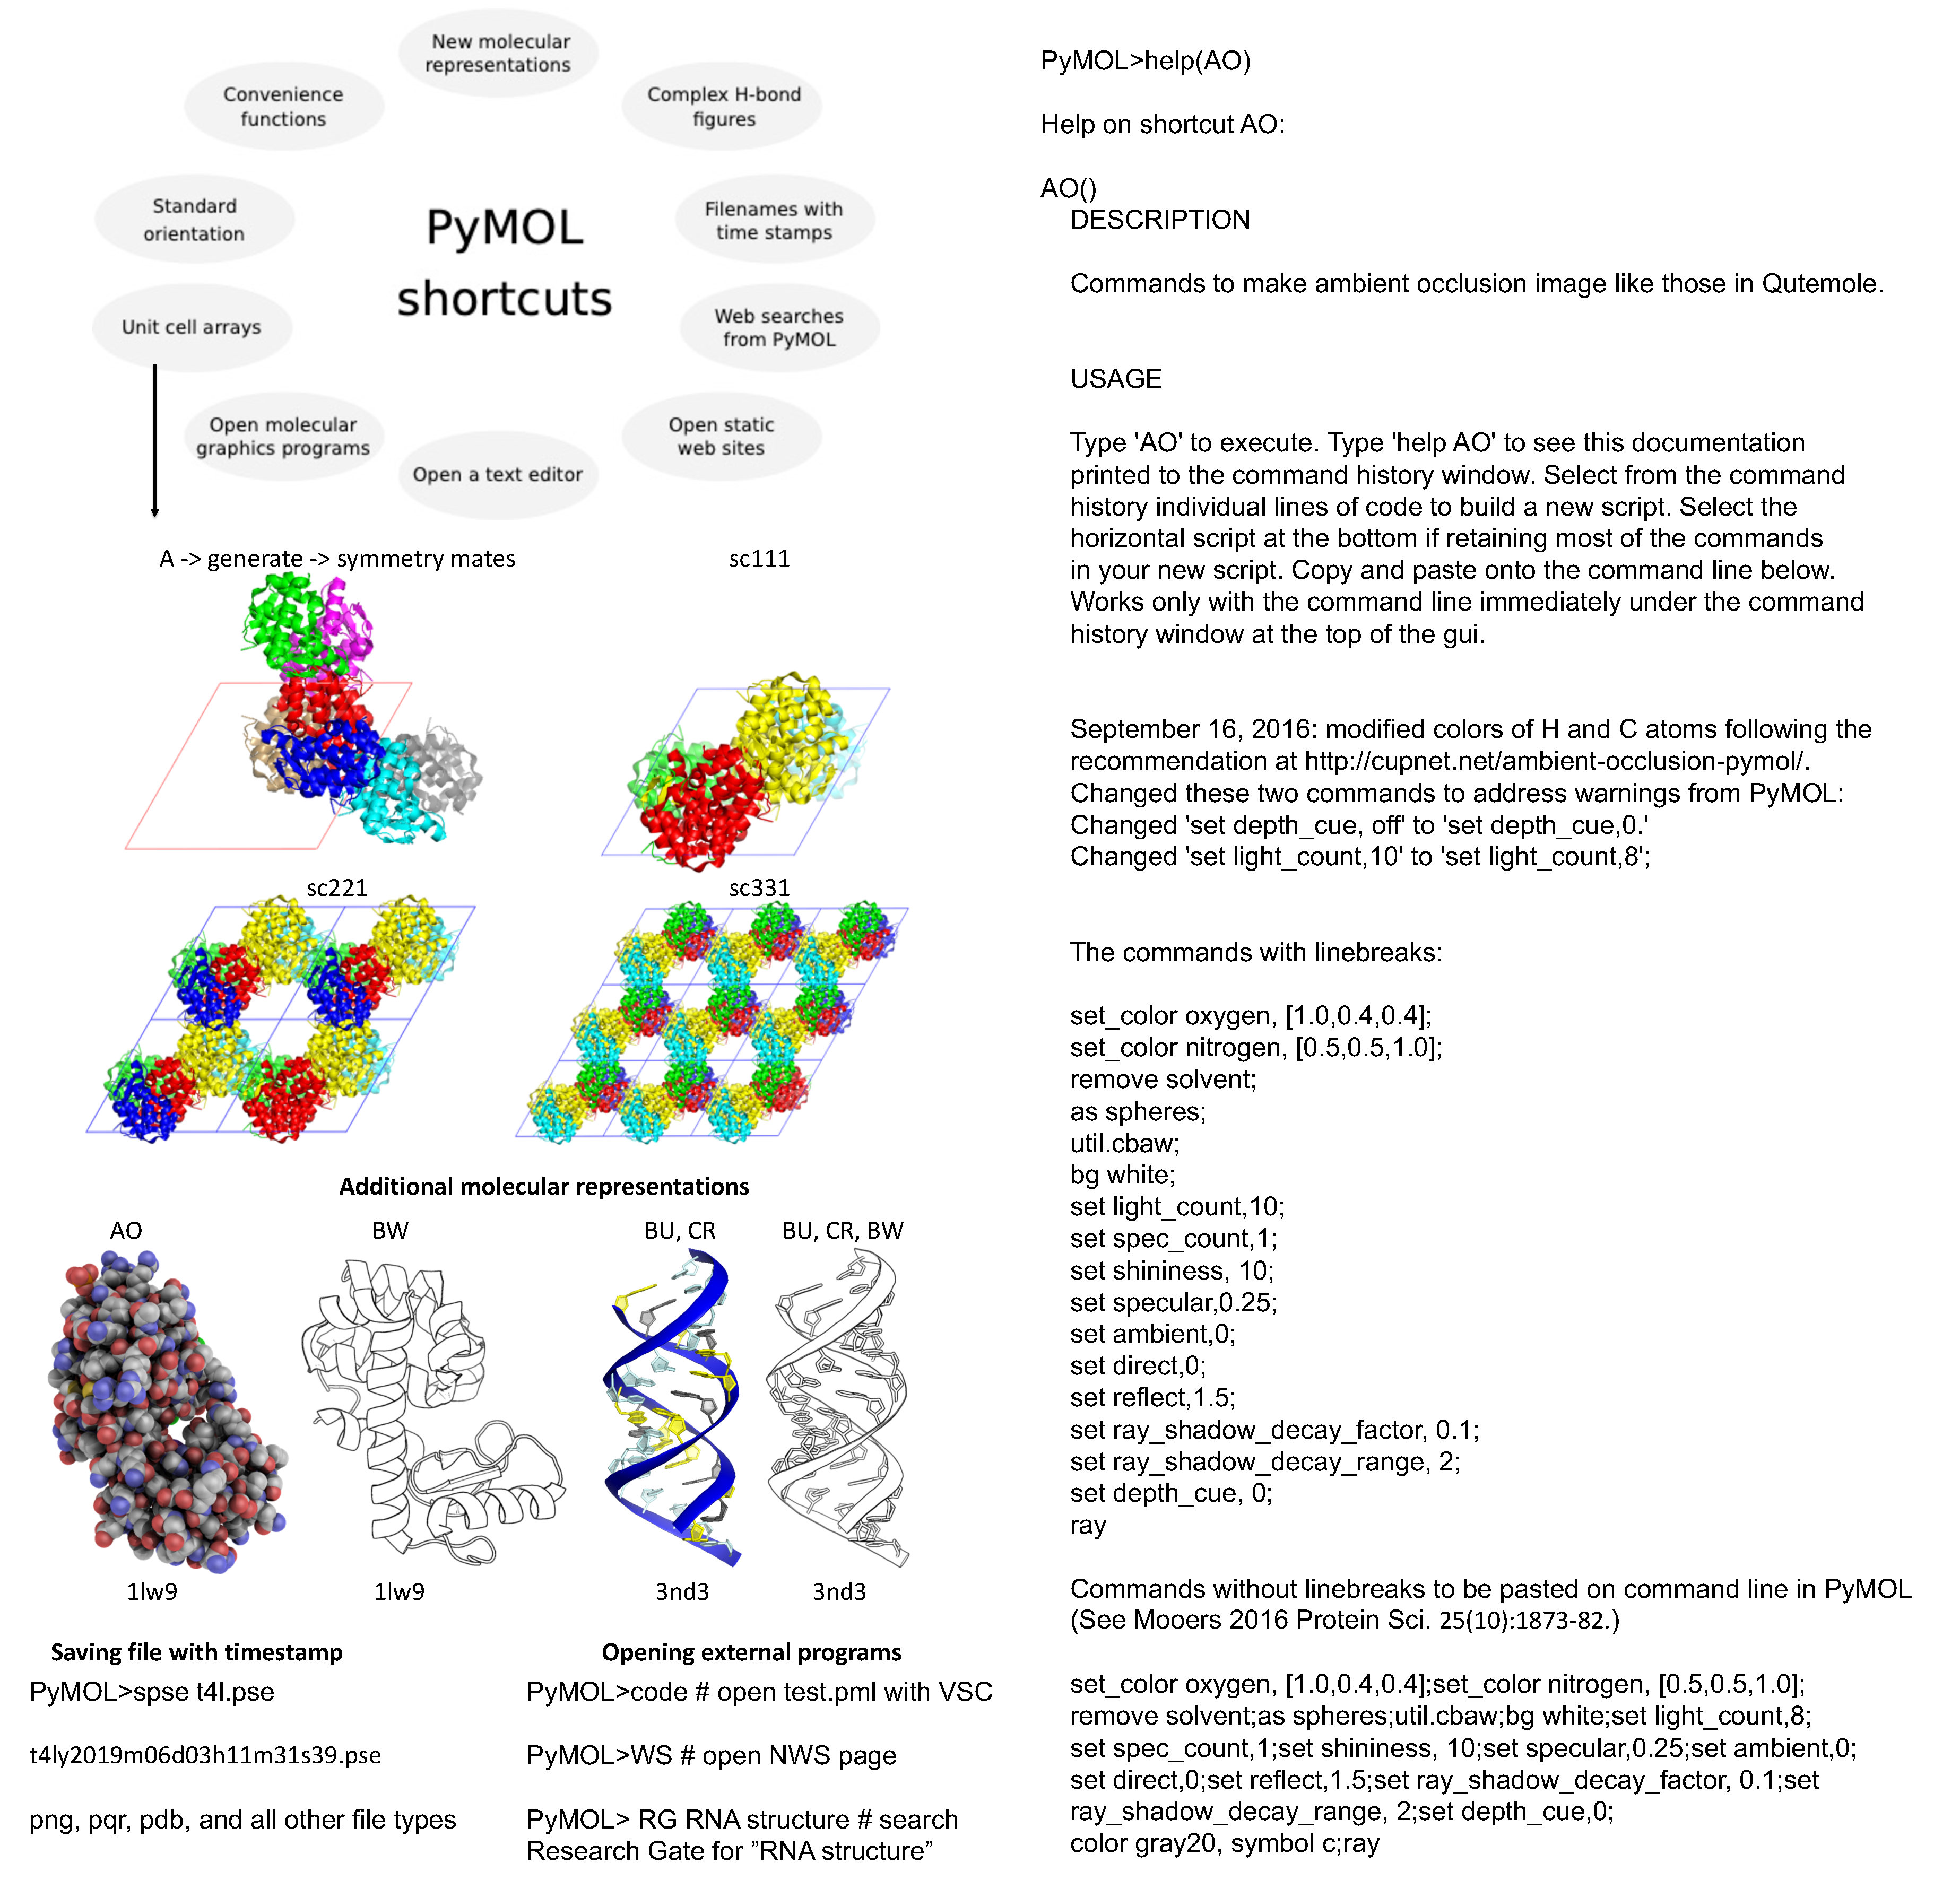
\includegraphics[scale=0.92]{./panel24by24OSB19.pdf}
\end{figure}
\end{center}

\begin{columns}[t,totalwidth=\textwidth]
\column{0.04\textwidth}
\column{0.2866\textwidth}

\begin{block}{Rationale}
\small{
\textbf{The need and gap:} 
The assembly of images of biomolecular structures for presentations and publication is often time consuming.
The automation of common but cumbersome tasks can save time.
The invoking of external programs from within PyMOL could also save more time because the viewport does not have to be moved aside. 
External programs include web browsers, text editors, image editors, word processors, email program, and calendars.
 
\vskip2ex
\textbf{Hypothesis:} Shortcuts ease structure analysis and image making with PyMOL. \\
\vskip2ex
\par}
\end{block}

\column{0.02\textwidth}
\column{0.2866\textwidth}

\begin{block}{Methods}
\small{
\begin{itemize}
    \item Shortcut == function in \url{pymolshortcuts.py}.
    \item Provide documentation for each function. 
    \item Use python modules external to PyMOL.
%    \item Only beautifulsoup4 (bs4) needs to be installed.
\end{itemize}
\par}
\end{block}

\begin{block}{Results}
\small{
\begin{itemize}
    \item SC prints list of shortcuts. 
    \item \textbf{help(<shortcut>)} prints docstring.
    \item Docstring includes pml code for reuse. 
    \item \textbf{webrowser,bs4,requests} for web searches. 
    \item \textbf{subprocess} opens external programs.
    \item Also see related \url{MooersLab/pymolsnips}
\end{itemize}
\par}
\end{block}

\column{0.02\textwidth}
\column{0.2866\textwidth}

\begin{block}{Summary}
\small{
\begin{itemize}
\item[\bullet]{More than 180 shortcuts.} 
\item[\bullet]{Access additional modules.}
\item[\bullet]{Access external programs.}
\item[\bullet]{Python 2.7 and 3.7 of PyMOL supported.}
\item[\bullet]{\url{http://github.com/MooersLab/pymolshortcuts}} 
\end{itemize}
\par}
\end{block}

\begin{block}{Funding}
\small{
\begin{itemize}
    \item Warren Delano Memorial Open-source PyMOL fellowship
    \item NSF MCB-1616865/1616845
    \item NIH/P20 GM103640 (PI Ann West)
\end{itemize}
\par}
\end{block}

% \begin{block}{Contact information}
% \small{
% blaine-mooers@ouhsc.edu
% \par}
% \end{block}

\column{0.04\textwidth}
\end{columns}
\end{frame}
\end{document}

	